\chapter{ကားရဲလ်နှင့် ရီကားဆစ်ဖ် ဖန်ရှင်များ}

ဖန်ရှင်တစ်ခုကနေ ‘အခြား’ ဖန်ရှင်တွေ ခေါ်သုံးတာကို အခန်း (၃) မှာ တွေ့ခဲ့ပြီးပါပြီ။ ဒါပေမဲ့ ဖန်ရှင်တစ်ခုက ၎င်းကိုယ်၎င်း ပြန်ခေါ်ထားတာကိုတော့ မကြုံဖူးသေးပါဘူး။ ဖန်ရှင်တွေဟာ ဆော့ဖ်ဝဲ အဆောက်အဦး တည်ဆောက်ရာမှာ မရှိမဖြစ်တဲ့ အခြေခံအုတ်ချပ်တွေလို့ ဆိုရမှာပါ။  ၎င်းကိုယ်တိုင်ကို ပြန်လည်အသုံးပြု၍ ဖန်ရှင်အုတ်ချပ်တစ်ခု ဖန်တီးလို့ ရနိုင်ပါမလား။ ဒီမေးခွန်းဟာ  ထူးဆန်းကောင်း ထူးဆန်းနေပါလိမ့်မယ်။ အခြေခံကျပြီး စိတ်ဝင်စားစရာကောင်းတဲ့ ဖီလော်ဆော်ဖီ မေးခွန်းလည်း ဖြစ်တယ်။

%\fEn{Recursive function} တွေဟာ  ခေါ် ဂျန်နရယ် ကွန်းဆက်ပ်မှာ အကျုံးဝင်တဲ့ ဥပမာတစ်ခုသာ ဖြစ်တယ်။ \fEnEmp{Recursion} ဆိုတာ 

%\fEnEmp{Recursion} ကတော့ ပိုပြီး ကျယ်ပြန့်တဲ့၊ ဂျန်နရယ်ကျတဲ့ ကွန်းဆက်ပ်ကို ရည်ညွှန်း‌ ဖော်ပြတာ ဖြစ်တယ်။ ရုပ်ပုံတစ်ခုမှာ \fEnEmp{recursion} သဘောတရား ပါဝင်နေရင် \fEn{recursive shape} ၊ ဖြစ်စဉ်တစ်ခုမှာ \fEnEmp{recursion} သဘောတရား ပါဝင်နေရင် \fEn{recursive process} ၊ အဓိပ္ပါယ်

ဖန်ရှင် သတ်မှတ်ချက်ထဲမှာ ၎င်းဖန်ရှင်ကိုယ်တိုင်ကို ပြန်ခေါ်လို့ ရပါတယ်။ ရီကားဆစ်ဖ် ဖန်ရှင် \fEn{(\textit{recursive function})} လို့ ခေါ်တယ်။ ရီကားဆစ်ဖ် ဖန်ရှင်တွေဟာ ဘီဂင်နာ ပရိုဂရမ်မာအတွက် နားလည်ဖို့ ခက်ခဲတဲ့ သဘောတရားအဖြစ် ယူဆကြတာကြောင့် စာအုပ် အတော်များများမှာ  နောက်ကျပြီး ဖော်ပြလေ့ရှိတယ်။ တကယ်က လူများစု ထင်/ပြောသလို နားမလည်နိုင်လောက်အောင် ရှုပ်ထွေး ခက်ခဲတဲ့ သဘောတရား မဟုတ်ပါဘူး။ သာမန်လူအားလုံး နားလည်နိုင်ပါတယ်။ ဒါကြောင့် စောစောစီးစီး အခုပဲ မိတ်ဆက်ပေးလိုက်ပါတယ်။ အကယ်၍ နားမလည်ခဲ့ရင်လည်း ပြဿနာမရှိပါဘူး။ အကြမ်းဖျဉ်းလောက် ဖတ်ကြည့်ပြီး နောက်လာမဲ့ အခန်းတွေကို ကျော်သွားနိုင်ပါတယ်။ နောင်တစ်ချိန်ကျမှ ပြန်လာဖတ်ပေါ့။

\section{ရီကားဆစ်ဖ် ဖန်ရှင် ဘယ်လို အလုပ်လုပ်လဲ}
 ရီကားဆစ်ဖ် ဖန်ရှင် ဥပမာတစ်ခုကို လေ့လာကြည့်ပါမယ်။ အောက်ဖော်ပြပါ ဖန်ရှင်ဟာ  ၎င်းကိုယ်တိုင်ကို ၎င်း ပြန်ခေါ်ထားတာ ဂရုပြုကြည့်ပါ။ \fEnEmp{recursive call} လို့ ကွန်းမန့်ရေးထားတဲ့ လိုင်းမှာပါ။
%
\setlength{\fboxsep}{0pt}
\begin{minted}[frame=\mintframe, framerule=\mintrule,framesep= \mintsep, xleftmargin=\xlftmargin
    , bgcolor=mintbgcolor,rulecolor=mintrulecolor
    , python3=true,escapeinside=ßß]{python}
def make_beeper_row():
    if front_is_clear():
        put_beeper()
        move()
        make_beeper_row() # ß\fEn{recursive call}ß
    else:
        put_beeper()
\end{minted}
%

ဒီဖန်ရှင်ကို ခေါ်လိုက်ရင် ဘာဆက်ဖြစ်မလဲဆိုတာ စိတ်ဝင်စားစရာပါ။  ဖန်ရှင်မစတင်မီ အနေအထားကို ပုံ  (\fRefNo{\ref{fig:mrofb_recur1}}) မှာ ကြည့်ပါ။ ဖန်ရှင်ကို ကနဦး  စခေါ်လိုက်တာမို့လို့ \fEnEmp{initial call} လို့ ရည်ညွှန်းပါမယ်။
%
\setlength{\fboxsep}{0pt}
\begin{minted}[frame=\mintframe, framerule=\mintrule,framesep= \mintsep, xleftmargin=\xlftmargin
    , bgcolor=mintbgcolor,rulecolor=mintrulecolor
    , python3=true,escapeinside=ßß]{python}
# ß\fEn{initial call}ß
make_beeper_row()
\end{minted}
%
\begin{figure}[htb!]
    {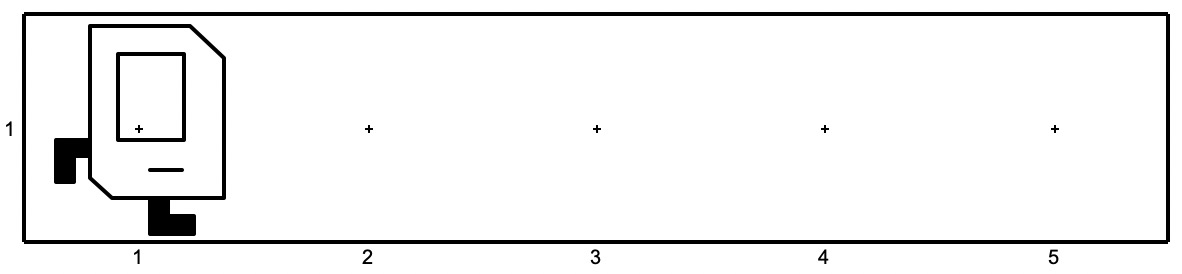
\includegraphics[scale=0.15]{images/ch04/mrofb/before.jpg}}
\caption{}
\label{fig:mrofb_recur1}
\end{figure}

ဖန်ရှင် စတင် လုပ်ဆောင်ပါမယ်။  ရှေ့မှာရှင်းနေတဲ့ အတွက် \fCode{if} ဘလောက်ကို လုပ်မှာပါ
%
\setlength{\fboxsep}{0pt}
\begin{minted}[frame=\mintframe, framerule=\mintrule,framesep= \mintsep, xleftmargin=\xlftmargin
    , bgcolor=mintbgcolor,rulecolor=mintrulecolor
    , python3=true,escapeinside=ßß]{python}
put_beeper()
move()
make_beeper_row() # ß\fEn{recursive call}ß
\end{minted}
%
ဘိပါချ၊ ရှေ့တိုး $\big\llbracket$ပုံ (\fRefNo{\ref{fig:mrofb_recur}}) (\fRefNo{\subref{fig:mrofb_recur2}})  ကြည့်ပါ$\big\rrbracket$ ပြီးရင် သူ့ကိုယ်သူ  ပြန်ခေါ်ထားတယ်။ ဒါဟာ ပထမဆုံး တစ်ကြိမ်ပါ။ ဖန်ရှင်ခေါ်ရင် ဖြစ်မြဲအတိုင်းပဲ ဖန်ရှင်နဲ့ သက်ဆိုင်တဲ့ ဘလောက်ကို ဆောက်ရွက်တာပေါ့။ ဒီတော့ \fCode{make\_beeper\_row} ဖန်ရှင်ဘလောက်ကိုပဲ တစ်ခါထပ်လုပ်မှာပါ။ ရှေ့မှာ ရှင်းနေတဲ့အတွက် \fCode{if} အပိုင်းကို လုပ်တယ်
%
\setlength{\fboxsep}{0pt}
\begin{minted}[frame=\mintframe, framerule=\mintrule,framesep= \mintsep, xleftmargin=\xlftmargin
    , bgcolor=mintbgcolor,rulecolor=mintrulecolor
    , python3=true,escapeinside=ßß]{python}
put_beeper()
move()
make_beeper_row() # ß\fEn{recursive call}ß
\end{minted}
%
ဘိပါချ၊ ရှေ့တိုး $\big\llbracket$ပုံ (\fRefNo{\ref{fig:mrofb_recur}}) (\fRefNo{\subref{fig:mrofb_recur3}})$\big\rrbracket$ ပြီး သူ့ကိုယ်သူ ပြန်ခေါ်ထားတဲ့ကိစ္စ တစ်ခါထပ်ဖြစ်ပြန်တယ်။ ဒါနဲ့ဆို နှစ်ကြိမ်။ ဖန်ရှင်ဘလောက် အလုပ် ပြန်လုပ်မယ်။ ရှေ့မှာရှင်းတယ်၊ \fCode{if} ကိုပဲ ထပ်လုပ်
%
\setlength{\fboxsep}{0pt}
\begin{minted}[frame=\mintframe, framerule=\mintrule,framesep= \mintsep, xleftmargin=\xlftmargin
    , bgcolor=mintbgcolor,rulecolor=mintrulecolor
    , python3=true,escapeinside=ßß]{python}
put_beeper()
move()
make_beeper_row() # ß\fEn{recursive call}ß
\end{minted}
%
ပုံ (\fRefNo{\ref{fig:mrofb_recur}}) (\fRefNo{\subref{fig:mrofb_recur4}}) နေရာရောက်ပြီး သူ့ကိုယ်သူ ထပ်ခေါ်ထားပြန်တယ်။ သုံးကြိမ်ရှိပြီ။ ဒီတစ်ခါလည်း \fCode{if} အပိုင်းပဲ ထပ်လုပ်
%
\setlength{\fboxsep}{0pt}
\begin{minted}[frame=\mintframe, framerule=\mintrule,framesep= \mintsep, xleftmargin=\xlftmargin
    , bgcolor=mintbgcolor,rulecolor=mintrulecolor
    , python3=true,escapeinside=ßß]{python}
put_beeper()
move()
make_beeper_row() # ß\fEn{recursive call}ß
\end{minted}
%
ရှေ့တိုးပြီးရင် နံရံပိတ်နေပြီ $\big\llbracket$ပုံ (\fRefNo{\ref{fig:mrofb_recur}}) (\fRefNo{\subref{fig:mrofb_recur5}})$\big\rrbracket$။ သူ့ကိုယ်သူ ခေါ်တယ်။ ရှေ့မှာ ပိတ်နေတဲ့အတွက် \fCode{else} အပိုင်းကို လုပ်မှာပါ။
%
\setlength{\fboxsep}{0pt}
\begin{minted}[frame=\mintframe, framerule=\mintrule,framesep= \mintsep, xleftmargin=\xlftmargin
    , bgcolor=mintbgcolor,rulecolor=mintrulecolor
    , python3=true,escapeinside=ßß]{python}
put_beeper()
\end{minted}
%
သူ့ကိုယ်သူ ပြန်ခေါ်တဲ့ကစ္စ ထပ်မဖြစ်တော့ဘူး။ ဒီမှာပဲ ပြီးဆုံးသွားတယ်။ ရီကားဆစ်ဖ် ဖန်ရှင် အလုပ်လုပ်ပုံ အခြေခံသဘောတရားက ဒါပါပဲ။ \fEn{loop} တွေ မသုံးဘဲ ပြန်ကျော့နေတဲ့ သဘောကို ရီကားဆစ်ဖ်ဖန်ရှင်မှာ တွေ့ရပါတယ်။ ဖန်ရှင်က သူ့ကိုယ်သူ (သို့ ကိုယ့်ကိုကိုယ်) ပြန်ခေါ်တာကို \fEnEmp{recursive call} လို့ခေါ်ပါတယ်။ ဒက်ဖ်နေးရှင်းအရ \fEn{recursive function} တွေမှာ \fEn{recursive call} အနည်းဆုံး တစ်ခု ပါရမှာ ဖြစ်ပါတယ်။


%ဒီတိုင်း ဆက်ကြည့်သွားရင် လေးကြိမ်မြောက် ရီကားဆစ်ဖ်‌ ကောလ်မှာ ရှေ့မှာနံရံပိတ်နေပြီ $\big\llbracket$ပုံ (\fRefNo{\ref{fig:mrofb_recur}}) (\fRefNo{\subref{fig:mrofb_recur4}})$\big\rrbracket$။ ဒီတော့ \fCode{else} အပိုင်း အလုပ်လုပ်ပါမယ်။ နောက်ဆုံး ဘိပါချမယ်။ ရီကားဆစ်ဖ်ကောလ် ဆက်မဖြစ်တော့ဘူး။ ဒီအခါ တစ်ဖက်စာမျက်နှာ \fEnEmpBf{*Initial Call*} ကွန်းမန့်အောက် ကနဦး \fCode{make\_beeper\_row} ဖန်ရှင်ကောလ်ကနေ စတင်ဖြစ်ပေါ်စေတဲ့ ရီးကားဆစ်ဖ်ဖန်ရှင် လုပ်ဆောင်မှုလည်း ပြီးဆုံးသွားမှာဖြစ်တယ်။

\begin{figure}[thb!]
    \newcommand{\figpctw}{0.49}
    \begin{subfigure}[t]{{\figpctw}\textwidth}
        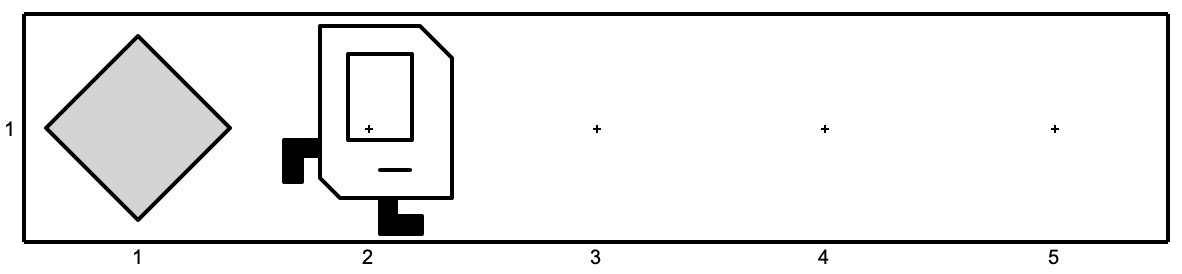
\includegraphics[scale=0.15]{images/ch04/mrofb/1st_iter.jpg}
        \caption{ပထမ တစ်ကျော့ပြီး}  
        \label{fig:mrofb_recur2}   
    \end{subfigure}
    \begin{subfigure}[t]{{\figpctw}\textwidth}
        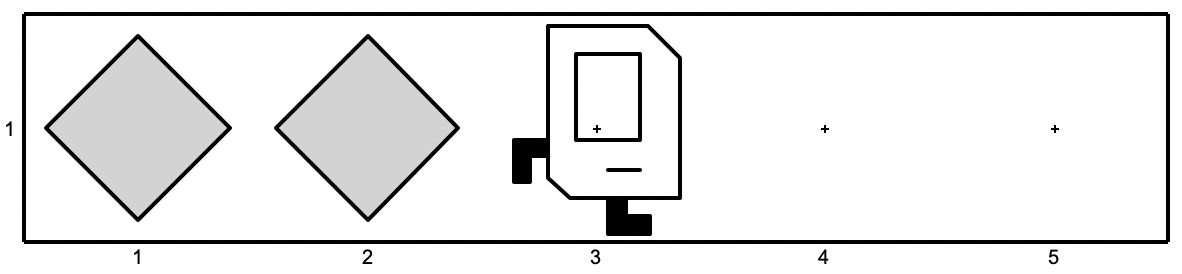
\includegraphics[scale=0.15]{images/ch04/mrofb/2nd_iter.jpg}
        \caption{ဒုတိယ တစ်ကျော့ပြီး}  
        \label{fig:mrofb_recur3}  
    \end{subfigure}
    \begin{subfigure}[t]{{\figpctw}\textwidth}
        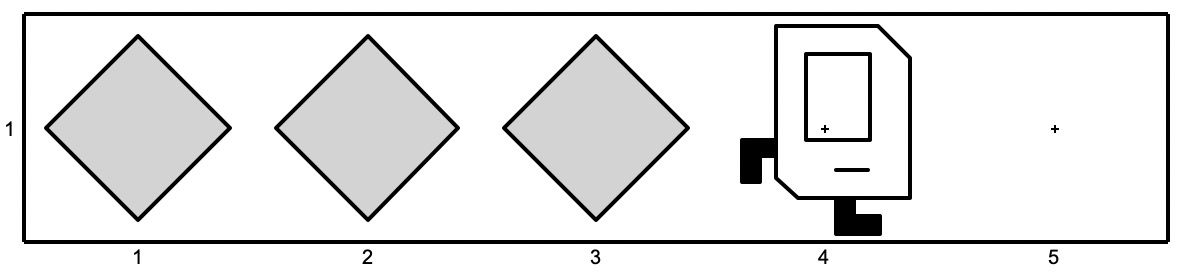
\includegraphics[scale=0.15]{images/ch04/mrofb/3rd_iter.jpg}
        \caption{တတိယ တစ်ကျော့ပြီး}  
        \label{fig:mrofb_recur4}  
    \end{subfigure}
    \begin{subfigure}[t]{{\figpctw}\textwidth}
        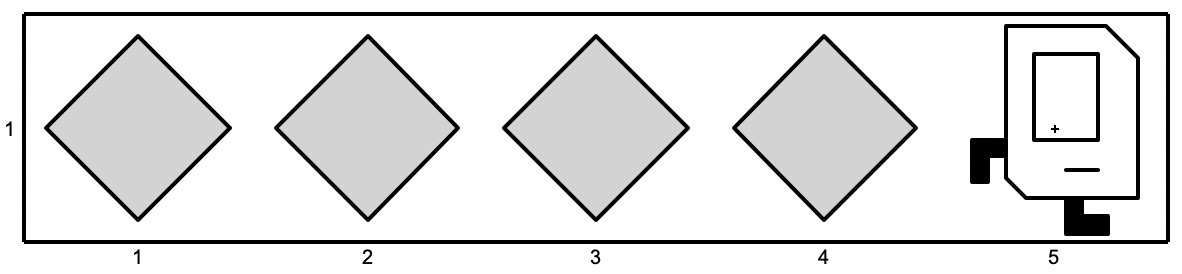
\includegraphics[scale=0.15]{images/ch04/mrofb/4th_iter.jpg}
        \caption{စတုတ္ထမြောက် ကျော့ပြီး}  
        \label{fig:mrofb_recur5}  
    \end{subfigure}
    \begin{subfigure}[t]{{\figpctw}\textwidth}
        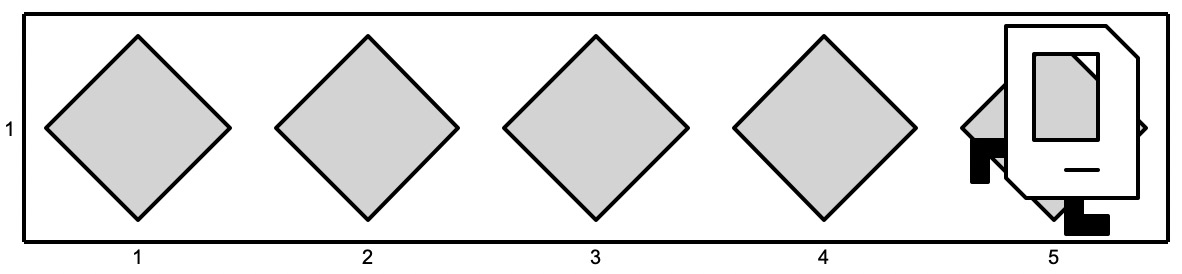
\includegraphics[scale=0.15]{images/ch04/mrofb/after.jpg}
        \caption{နောက်ဆုံး \fCptCodeBf{putBeeper} လုပ်ပြီး}    
        \label{fig:mrofb_recur6}
    \end{subfigure}
    \caption{}
    \label{fig:mrofb_recur}
\end{figure}


%
\setlength{\fboxsep}{0pt}
\begin{minted}[frame=\mintframe, framerule=\mintrule,framesep= \mintsep, xleftmargin=\xlftmargin
    , bgcolor=mintbgcolor,rulecolor=mintrulecolor
    , python3=true,escapeinside=ßß]{python}
def make_beeper_row():
    if front_is_clear():ß\tikzmark{a2}ß
        put_beeper()
        move()
        make_beeper_row()ß\tikzmark{a3}ß
    else:
        put_beeper()ß\tikzmark{a4}ß

make_beeper_row()ß\tikzmark{a1}ß
\end{minted}
%
\begin{tikzpicture}[
  remember picture,
  overlay,
  annotation/.style={
    inner sep=0pt,
    outer sep=0pt,
    outer xsep=0mm,
    fill=yellow!80!black,
    text width=5cm
  },
  >={Stealth[inset=0pt, angle=30:7pt]}
]
\draw[->, thick] ([yshift=0ex] pic cs:a1) -- ++(3,0) |- ([yshift=1.4ex]pic cs:a2);%
\draw[->, thin,blue] ([yshift=0ex] pic cs:a3) -- ++(1,0) |- ([yshift=0.5ex] pic cs:a2);%
\draw[->, thin,blue] ([yshift=1.2ex] pic cs:a3) -- ++(.7,0) |- ([yshift=-.4ex] pic cs:a2);%
\draw[->, thin,red] ([yshift=0.5ex] pic cs:a4) -- ++(.7,0) |- ([yshift=1.2ex] pic cs:a1);%
\end{tikzpicture}%
\btwntikzannoandpar

ရီကားဆစ်ဖ်ကောလ် ဖြစ်တာကို စိတ်ကူးပုံဖော်ကြည့်ဖို့ ပြထားတာပါ။ အပြင်ဆုံး မြှားအနက်က ကန\allowbreak ဦး ဖန်ရှင်ကောလ် စတင်တာဖြစ်‌ပေါ်တာကို ဖော်ပြတယ်။ ရီကားဆစ်ဖ်ကောလ် မဟုတ်သေးဘူး။ မြှားအပြာက ရီကားဆစ်ဖ်ကောလ်ကြောင့် ဖန်ရှင်အစ ပြန်ရောက်သွားတာကို ပြတယ်။ ပထမနဲ့ ဒုတိယ ရီကားဆစ်ဖ်ကောလ် နှစ်ခုအတွက်ပြထားတာပါ။ ရှေ့က ဥပမာအတွက် မြှားအပြာ လေးခု ရှိရမှာပါ (ရီကားဆစ်ဖ်ကောလ် လေးကြိမ်အတွက်)။  မြှားအပြာ နောက်ထပ် နှစ်ခုရှိတယ် မှတ်ယူပါ (ပုံမှာထပ်ထည့်ရင် ကြပ်ညပ်ပြီး ကြည့်ရရှုပ်လို့ မဆွဲပြတာ)။ လေးကြိမ်မြောက်မှာ ရီကားဆစ်ဖ်ကောလ် ထပ်မဖြစ်တော့ဘူး (\fCode{if} အပိုင်းကို မလုပ်တော့တဲ့အတွက်)။ ဘိပါချပြီး ဖန်ရှင်ကောလ် စခဲ့တဲ့နေရာကို ပြန်ရောက် သွားမယ် (မြှားအနီ)။ ဘယ်လို ပြန်ရောက်သွားတာလဲ ဆက်ကြည့်ရအောင်။

\subsection*{နောက်ဆုံး ရီကားဆစ်ဖ်ကောလ်မှ ပြန်လာခြင်း}
နောက်ဆုံး ရီကားဆစ်ဖ်ကောလ်ကနေ မူလ ဖန်ရှင်ခေါ်ခဲ့တဲ့ နေရာကို ဘယ်လိုပြန်ရောက်သွားတာလဲ။ ဒီကိစ္စနားလည်ဖို့ ဖန်ရှင် \fEnEmp{return} ပြန်ခြင်းအကြောင်း အရင်ကြည့်ရပါမယ်။ ဖန်ရှင်ကောလ် လုပ်ဆောင်တဲ့အခါ အဲဒီဖန်ရှင်နဲ့ သက်ဆိုင်တဲ့ ဘလောက်ဆီကို ခုန်ကျော် ရောက်ရှိသွားမှာပါ။ ဖန်ရှင်ဘလောက်ကို လုပ်ဆောင်ပြီး ခေါ်ခဲ့တဲ့ နေရာကို ပြန်လည်ရောက်ရှိသွားမှာ ဖြစ်တယ်။ ဒီဖြစ်စဉ်ကို ဖန်ရှင် \fEn{return} ပြန်တယ်လို့ ပြောပါတယ်။
%
\setlength{\fboxsep}{0pt}
\begin{minted}[frame=\mintframe, framerule=\mintrule,framesep= \mintsep, xleftmargin=\xlftmargin
    , bgcolor=mintbgcolor,rulecolor=mintrulecolor
    , python3=true,escapeinside=ßß]{python}
def main():
    turn_right()ß\tikzmark{b1}ß
    move()
    turn_right()
    move()

def turn_right():
    turn_left()ß\tikzmark{b2}ß
    turn_left()
    turn_left()ß\tikzmark{b3}ß
\end{minted}
\begin{tikzpicture}[
  remember picture,
  overlay,
  annotation/.style={
    inner sep=0pt,
    outer sep=0pt,
    outer xsep=1mm,
    fill=yellow!80!black,
    text width=5cm
  },
  >={Stealth[inset=0pt, angle=30:7pt]}
]
\draw[->, thin] (pic cs:b1)  ++(0,1.2ex) -- ++(1,0) |- ([yshift=0.5ex] pic cs:b2);
\draw[->, thin, red] (pic cs:b3)  ++(0,.5ex) -- ++(2,0) |- (pic cs:b1);
\end{tikzpicture}%
ပထမ \fCode{turn\_right} ကောလ် လုပ်ဆောင်တဲ့အခါ ကောလ်လုပ်တဲ့ နေရာကနေ \fCode{turn\_right} ဖန်ရှင်ထဲကို \fEn{jump} လုပ်ပြီး ရောက်သွားတယ်။ မြှားအနက်နဲ့ ပြထားတယ်။ ဖန်ရှင်ဘလောက် လုပ်ဆောင်ပြီးတဲ့အခါ ခေါ်ခဲ့တဲ့နေရာ \fCode{main} ဖန်ရှင်ထဲ ပြန်ရောက်သွားတယ် (မြှားအနီ)။ ဒုတိယ \fCode{turn\_right} လည်း ထိုနည်းတူစွာပဲ ဖြစ်ပါတယ်။


%
\setlength{\fboxsep}{0pt}
\begin{minted}[frame=\mintframe, framerule=\mintrule,framesep= \mintsep, xleftmargin=\xlftmargin
    , bgcolor=mintbgcolor,rulecolor=mintrulecolor
    , python3=true,escapeinside=ßß]{python}
def main():
    turn_right()
    move()
    turn_right()ß\tikzmark{c1}ß
    move()

def turn_right():
    turn_left()ß\tikzmark{c2}ß
    turn_left()
    turn_left()ß\tikzmark{c3}ß
\end{minted}
\begin{tikzpicture}[
  remember picture,
  overlay,
  annotation/.style={
    inner sep=0pt,
    outer sep=0pt,
    outer xsep=1mm,
    fill=yellow!80!black,
    text width=5cm
  },
  >={Stealth[inset=0pt, angle=30:7pt]}
]
\draw[->, thin] (pic cs:c1)  ++(0,1.2ex) -- ++(1,0) |- ([yshift=0.5ex] pic cs:c2);
\draw[->, thin, red] (pic cs:c3)  ++(0,.5ex) -- ++(2,0) |- (pic cs:c1);
\end{tikzpicture}
\btwntikzannoandpar

နှစ်ဆင့်၊ သုံးဆင့် ဖန်ရှင်ကောလ်တွေမှာလည်း ဒီသဘောတရား အတိုင်းပါပဲ။ အောက်ဖော်ပြပါ ပရိုဂရမ်ကုဒ်ကို ကြည့်ပါ။ \fCode{main} ဖန်ရှင်ထဲကနေ \fCode{do\_tricks} ဆီကို ရောက်သွားမယ်။ \fCode{do\_tricks} ထဲကနေ \fCode{put\_two} ထဲကို ရောက်သွားမယ်။ 
%
\setlength{\fboxsep}{0pt}
\begin{minted}[frame=\mintframe, framerule=\mintrule,framesep= \mintsep, xleftmargin=\xlftmargin
    , bgcolor=mintbgcolor,rulecolor=mintrulecolor
    , python3=true,escapeinside=ßß]{python}
def main():
    do_tricks()ß\tikzmark{d1}ß
    move()

def do_tricks():
    move()ß\tikzmark{d2}ß
    put_two()ß\tikzmark{d3}ß
    turn_left()
    move()ß\tikzmark{d4}ß

def put_two():
    put_beeper()ß\tikzmark{d5}ß
    put_beeper()ß\tikzmark{d6}ß
\end{minted}
\begin{tikzpicture}[
  remember picture,
  overlay,
  annotation/.style={
    inner sep=0pt,
    outer sep=0pt,
    outer xsep=1mm,
    fill=yellow!80!black,
    text width=5cm
  },
  >={Stealth[inset=0pt, angle=30:7pt]}
]
\draw[->, thin] (pic cs:d1)  ++(0,1.2ex) -- ++(1,0) |- ([yshift=0.5ex] pic cs:d2);
\draw[->, thin] (pic cs:d3)  ++(0,1.2ex) -- ++(1,0) |- ([yshift=0.5ex] pic cs:d5);
\draw[->, thin, red] (pic cs:d6)  ++(0,.5ex) -- ++(0.7,0) |- (pic cs:d3);
\draw[->, thin, red] (pic cs:d4)  ++(0,.5ex) -- ++(2.1,0) |- (pic cs:d1);
\end{tikzpicture}%
%

\fCode{put\_two} ပြီးသွားတဲ့အခါ \fCode{do\_tricks} ထဲ ပြန်ရောက်သွားမယ်။ \fCode{turn\_left}\fEn{,} \fCode{move} ဆက်လုပ်ပြီး \fCode{do\_tricks} ခေါ်ခဲ့တဲ့နေရာ \fCode{main} ထဲ ပြန်ရောက်သွားမယ်။ နောက်ဆုံး \fCode{main} ထဲက \fCode{move}  ကို ဆက်လုပ်ပါတယ်။

ဖန်ရှင် အဆင့်ဆင့် ခေါ်ထားတဲ့အခါ နောက်ဆုံးခေါ်တဲ့ ဖန်ရှင်က အရင်ဆုံး \fEn{return} ပြန်ပါတယ်။ \fCode{main} ကနေ \fCode{do\_tricks} ကိုခေါ်၊ \fCode{do\_tricks} ကနေ \fCode{put\_two} ကိုခေါ်ထားရင် \fCode{put\_two} ကနေ \fCode{do\_tricks} ဆီကို အရင် \fEn{return} ပြန်တယ်။ ပြီးတော့မှ \fCode{do\_tricks} ကနေ \fCode{main} ကို ပြန်ရောက်မှာပါ။ ဒီသဘောအရ \fCode{put\_two} \fEn{return} မပြန်မချင်း \fCode{do\_tricks} ဖန်ရှင်မပြီးသေးဘူး။ \fCode{put\_two} ကနေပြန်လာပြီးမှ ကျန်တဲ့ \fCode{turn\_left}\fEn{,} \fCode{move} ဆက်လုပ်တယ်။ ပြီးတော့မှ \fCode{do\_tricks} ဖန်ရှင်က \fEn{return} ပြန်ပါတယ်။ 


ရီကားဆစ်ဖ် ဖန်ရှင်ကောလ်တွေ ဘယ်လို \fEn{return} ပြန်လဲ။ ရှေ့ကလို မြှားတွေနဲ့ ဆွဲပြလို့ ရပေမဲ့ ကြည့်ရတာ ရှုပ်ရှက်ခတ်နေမှာပါ။ အခုလို မြင်ကြည့်ရင် ပိုရှင်းပါတယ်။
%
\setlength{\fboxsep}{0pt}
\begin{minted}[frame=\mintframe, framerule=\mintrule,framesep= \mintsep, xleftmargin=\xlftmargin
    , bgcolor=mintbgcolor,rulecolor=mintrulecolor
    , python3=true,escapeinside=ßß]{python}
# ß\fEn{initial call}ß
make_beeper_row()ß\tikzmarknode{e1}ß
    # ß\fEn{1\textsuperscript{\fEn{st}} recur}ß
    make_beeper_row()ß\tikzmarknode{e2}ß
        # ß\fEn{2\textsuperscript{\fEn{nd}} recur}ß
        make_beeper_row()ß\tikzmarknode{e3}ß
            # ß\fEn{3\textsuperscript{\fEn{rd}} recur}ß
            make_beeper_row()ß\tikzmarknode{e4}ß
                # ß\fEn{4\textsuperscript{\fEn{th}} recur}ß
                make_beeper_row()ß\tikzmarknode{e5}ß
\end{minted}
\begin{tikzpicture}[
  remember picture,
  overlay,
  annotation/.style={
    inner sep=0pt,
    outer sep=0pt,
    outer xsep=1mm,
    fill=yellow!80!black,
    text width=5cm
  },
  >={Stealth[inset=0pt, angle=30:7pt]}
]
\draw[->, thin] (pic cs:e1)  ++(0,.3ex) .. controls ([xshift=1.1cm,yshift=-.11cm]pic cs:e1) and ([xshift=.5cm,yshift=.5cm]pic cs:e2) ..  ([yshift=1.2ex] pic cs:e2);
\draw[->, thin] (pic cs:e2)  ++(0,0ex) .. controls ([xshift=1.1cm,yshift=-.11cm]pic cs:e2) and ([xshift=.5cm,yshift=.5cm]pic cs:e3) ..  ([yshift=1.2ex] pic cs:e3);
\draw[->, thin] (pic cs:e3)  ++(0,0ex) .. controls ([xshift=1.1cm,yshift=-.11cm]pic cs:e3) and ([xshift=.5cm,yshift=.5cm]pic cs:e4) ..  ([yshift=1.2ex] pic cs:e4);
\draw[->, thin] (pic cs:e4)  ++(0,0ex) .. controls ([xshift=1.1cm,yshift=-.11cm]pic cs:e4) and ([xshift=.5cm,yshift=.5cm]pic cs:e5) ..  ([yshift=.7ex] pic cs:e5);
\draw[->, thin, red] (pic cs:e5)  ++(0,0ex) .. controls ([xshift=1.7cm,yshift=.4cm]pic cs:e5) and ([xshift=1cm,yshift=.2cm]pic cs:e4) ..  ([yshift=.5ex] pic cs:e4);
\draw[->, thin, red] (pic cs:e4)  ++(0,1ex) .. controls ([xshift=1.7cm,yshift=.4cm]pic cs:e4) and ([xshift=1cm,yshift=.2cm]pic cs:e3) ..  ([yshift=.5ex] pic cs:e3);
\draw[->, thin, red] (pic cs:e3)  ++(0,1ex) .. controls ([xshift=1.7cm,yshift=.4cm]pic cs:e3) and ([xshift=1cm,yshift=.2cm]pic cs:e2) ..  ([yshift=.5ex] pic cs:e2);
\draw[->, thin, red] (pic cs:e2)  ++(0,1ex) .. controls ([xshift=1.7cm,yshift=.4cm]pic cs:e2) and ([xshift=1cm,yshift=.2cm]pic cs:e1) ..  ([yshift=.7ex] pic cs:e1);
%([yshift=0.1em]a.north) to[bend left] ([yshift=0.1em]b.north);}
\end{tikzpicture}%
\btwntikzannoandpar

မြှားအနက်တွေက ဖန်ရှင်ကောလ်  တစ်ဆင့်ပြီးတစ်ဆင့် ဖြစ်တာကို ပြတာပါ။ အထက်မှအောက် အစီ\allowbreak အစဉ်အတိုင်း ဖြစ်ပါတယ်။ ‌လေးကြိမ်မြောက်မှာ နောက်ထပ် ရီကားဆစ်ဖ်ကောလ် ထပ်မဖြစ်တော့ဘဲ နောက်ဆုံး ရီကားဆစ်ဖ်ကောလ်က အရင်ဆုံး \fEn{return} စပြန်ပါတယ် (အောက်ဆုံး မြှားအနီနဲ့ ပြထား)။ ဒီအခါ တတိယ ရီကားဆစ်ဖ်ကောလ်ကို ပြန်ရောက်သွားမှာပါ။ ဒီအတိုင်း တစ်ဆင့်ပြီးတစ်ဆင့် အထက်ကို \fEn{return} ပြန်ပြီး နောက်ဆုံးမှာ ပထမဆုံး ခေါ်ခဲ့တဲ့နေရာ ပြန်ရောက်သွားမှာပါ။ (အခုပြထားတာကို တကယ့် \fEn{Python} ကုဒ် အနေနဲ့ မယူဆရပါ၊ ဖြစ်စဉ် နားလည်အောင် ပြခြင်းသာဖြစ်ပါတယ်)။ နဲနဲပြင်ထားတဲ့ \fCode{make\_beeper\_\allowbreak row}  ဗားရှင်းမှာ \fEn{return} ပြန်တဲ့ ဖြစ်စဉ်ကို ကြည့်ရအောင်။ 

%
\setlength{\fboxsep}{0pt}
\begin{minted}[frame=\mintframe, framerule=\mintrule,framesep= \mintsep, xleftmargin=\xlftmargin
    , bgcolor=mintbgcolor,rulecolor=mintrulecolor
    , python3=true,escapeinside=ßß]{python}
make_beeper_row()
\end{minted}
%
\betweenminted{\medskipamount}
%
\setlength{\fboxsep}{0pt}
\begin{minted}[frame=\mintframe, framerule=\mintrule,framesep= \mintsep, xleftmargin=\xlftmargin
    , bgcolor=mintbgcolor,rulecolor=mintrulecolor
    , python3=true,escapeinside=ßß]{python}
def make_beeper_row():
    if front_is_clear():
        put_beeper()
        move()
        make_beeper_row()
        turn_left()
        move()
    else:
        put_beeper()
\end{minted}
%
\btwntikzannoandpar

\fCode{if}  အပိုင်း ရီကားဆစ်ဖ်ကောလ်ပြီး  \fCode{turn\_\allowbreak left} နဲ့ \fCode{move} ထပ်ဖြည့်ထားတာ။  ရီကားဆစ်ဖ်ကောလ် \fEn{return} ပြန်လာပြီးမှ ဒီနှစ်ခု ဆက်လုပ်မှာပါ။  နောက်ဆုံး ရီကားဆစ်ဖ်ကောလ်က \fEn{return} စဖြစ်တယ်။ ဒီတော့မှ တတိယအောက် \fCode{turn\_\allowbreak left} နဲ့ \fCode{move} ကို လုပ်ဆောင်မှာပါ။ ပြီးမှ တတိယကောလ် \fEn{return} ပြန်တယ်။ ဒီအတိုင်း အထက်ကို တက်သွားပြီး ကျန်နေသေးတဲ့ စတိတ်မန့်တွေကို လုပ်ဆောင်ပါတယ်။ ပထမဆုံးကောလ်အောက် ကျန်နေတာတွေ နောက်ဆုံးကျမှ ပြီးမှာပါ။

%
\setlength{\fboxsep}{0pt}
\begin{minted}[frame=\mintframe, framerule=\mintrule,framesep= \mintsep, xleftmargin=\xlftmargin
    , bgcolor=mintbgcolor,rulecolor=mintrulecolor
    , python3=true,escapeinside=ßß]{python}
# ß\fEn{initial call}ß
make_beeper_row()ß\tikzmarknode{f1}ß
    # ß\fEn{1\textsuperscript{\fEn{st}} recur}ß
    make_beeper_row()ß\tikzmarknode{f2}ß
    turn_left()
    move()ß\tikzmarknode{f2a}ß
        # ß\fEn{2\textsuperscript{\fEn{nd}} recur}ß
        make_beeper_row()ß\tikzmarknode{f3}ß
        turn_left()
        move()ß\tikzmarknode{f3a}ß
            # ß\fEn{3\textsuperscript{\fEn{rd}} recur}ß
            make_beeper_row()ß\tikzmarknode{f4}ß
            turn_left()
            move()ß\tikzmarknode{f4a}ß
                # ß\fEn{4\textsuperscript{\fEn{th}} recur}ß
                make_beeper_row()ß\tikzmarknode{f5}ß
\end{minted}
\begin{tikzpicture}[
  remember picture,
  overlay,
  annotation/.style={
    inner sep=0pt,
    outer sep=0pt,
    outer xsep=1mm,
    fill=yellow!80!black,
    text width=5cm
  },
  >={Stealth[inset=0pt, angle=30:7pt]}
]
\draw[->, thin] (pic cs:f1)  ++(0,.3ex) .. controls ([xshift=1.1cm,yshift=-.11cm]pic cs:f1) and ([xshift=.5cm,yshift=.5cm]pic cs:f2) ..  ([yshift=1.2ex] pic cs:f2);
\draw[->, thin] (pic cs:f2)  ++(0,0ex) .. controls ([xshift=1.1cm,yshift=-.11cm]pic cs:f2) and ([xshift=.5cm,yshift=.5cm]pic cs:f3) ..  ([yshift=1.2ex] pic cs:f3);
\draw[->, thin] (pic cs:f3)  ++(0,0ex) .. controls ([xshift=1.1cm,yshift=-.11cm]pic cs:f3) and ([xshift=.5cm,yshift=.5cm]pic cs:f4) ..  ([yshift=1.2ex] pic cs:f4);
\draw[->, thin] (pic cs:f4)  ++(0,0ex) .. controls ([xshift=1.1cm,yshift=-.11cm]pic cs:f4) and ([xshift=.5cm,yshift=.5cm]pic cs:f5) ..  ([yshift=.7ex] pic cs:f5);
\draw[->, thin, red] (pic cs:f5)  ++(0,0ex) .. controls ([xshift=1.7cm,yshift=.4cm]pic cs:f5) and ([xshift=1cm,yshift=.2cm]pic cs:f4) ..  ([yshift=.5ex] pic cs:f4);
\draw[->, thin, red] (pic cs:f4a)  ++(0,.5ex) .. controls ([xshift=4.5cm,yshift=.7cm]pic cs:f4a) and ([xshift=1cm,yshift=.2cm]pic cs:f3) ..  ([yshift=.5ex] pic cs:f3);
\draw[->, thin, red] (pic cs:f3a)  ++(0,.5ex) .. controls ([xshift=4.5cm,yshift=.7cm]pic cs:f3a) and ([xshift=1cm,yshift=.2cm]pic cs:f2) ..  ([yshift=.5ex] pic cs:f2);
\draw[->, thin, red] (pic cs:f2a)  ++(0,.5ex) .. controls ([xshift=4.5cm,yshift=.7cm]pic cs:f2a) and ([xshift=1cm,yshift=.2cm]pic cs:f1) ..  ([yshift=.5ex] pic cs:f1);
%([yshift=0.1em]a.north) to[bend left] ([yshift=0.1em]b.north);}
\end{tikzpicture}


ရီကားဆစ်ဖ်ကောလ် နှစ်ခါပဲ ဖြစ်မယ်ဆိုရင် အောက်ပါအတိုင်း မြင်ကြည့်လို့ ရပါတယ်။ မြှားအပြာနှစ်ခုက ရီကားဆစ်ဖ်ကောလ်ဖြစ်တာ။ ဒုတိယကောလ်က ဘိပါချပြီး (\fCode{else} အပိုင်း) အရင် \fEn{return} မယ်။ အထက်ကို ညွှန်တဲ့ မြှားအနီကို ကြည့်ပါ။ ဘယ်လှည့်၊ ရှေ့တိုးပြီး ပထမ ကောလ်က နောက်မှ \fEn{initial call} လုပ်ခဲ့တဲ့ဆီ ပြန်ရောက်တာ။ အောက်ကိုညွှန်တဲ့ မြှားအနီကို ကြည့်ပါ။
%
\setlength{\fboxsep}{0pt}
\begin{minted}[frame=\mintframe, framerule=\mintrule,framesep= \mintsep, xleftmargin=\xlftmargin
    , bgcolor=mintbgcolor,rulecolor=mintrulecolor
    , python3=true,escapeinside=ßß]{python}
def make_beeper_row():
    if front_is_clear():ß\tikzmark{g2}ß
        put_beeper()
        move()
        make_beeper_row()ß\tikzmark{g3}ß
        turn_left()
        move()ß\tikzmark{g3a}ß
    else:
        put_beeper()ß\tikzmark{g4}ß

# ß\fEn{initial call}ß
make_beeper_row()ß\tikzmark{g1}ß
\end{minted}
%
\begin{tikzpicture}[
  remember picture,
  overlay,
  annotation/.style={
    inner sep=0pt,
    outer sep=0pt,
    outer xsep=0mm,
    fill=yellow!80!black,
    text width=5cm
  },
  >={Stealth[inset=0pt, angle=30:7pt]}
]
\draw[->, thick] ([yshift=1.2ex] pic cs:g1) -- ++(3,0) |- ([yshift=1.4ex]pic cs:g2);%
\draw[->, thin,blue] ([yshift=.5ex] pic cs:g3) -- ++(1,0) |- ([yshift=0.5ex] pic cs:g2);%
\draw[->, thin,blue] ([yshift=1.4ex] pic cs:g3) -- ++(.7,0) |- ([yshift=-.4ex] pic cs:g2);%
\draw[->, thin,red] ([yshift=0.5ex] pic cs:g4) -- ++(1.5,0) |- ([yshift=-.4ex] pic cs:g3);%
\draw[->, thin,red] ([yshift=0.5ex] pic cs:g3a) -- ++(1.5,0) |- ([yshift=0ex] pic cs:g1);%
\end{tikzpicture}%
\btwntikzannoandpar

ရီကားဆစ်ဖ် ဖန်ရှင်အကြောင်း လေ့လာတဲ့အခါ ဘီဂင်နာအများစု ကြေကြေညက်ညက် နားလည်ဖို့အတွက် အခက်အခဲဆုံးတစ်ခုက \fEn{return} ပြန်တဲ့ သဘောတရားပါပဲ။  များများစဉ်းစား၊ များများလေ့ကျင့်ရင် ဒီအခက်အခဲ ကျော်ဖြတ်နိုင်မှာပါ။ \fCode{if...else} အပြီးမှာ \fCode{put\_beeper} လေးတစ်ခုပဲ ထပ်ဖြည့်လိုက်ရင် ဘယ်လိုဖြစ်မလဲ။
%
\setlength{\fboxsep}{0pt}
\begin{minted}[frame=\mintframe, framerule=\mintrule,framesep= \mintsep, xleftmargin=\xlftmargin
    , bgcolor=mintbgcolor,rulecolor=mintrulecolor
    , python3=true,escapeinside=ßß]{python}
# File: make_beeper_row2.py
def make_beeper_row():
    if front_is_clear():
        put_beeper()
        move()
        make_beeper_row()
        turn_left()
        move()
    else:
        put_beeper()
    put_beeper()

# ß\fEn{initial call}ß
make_beeper_row()
\end{minted}
ပုံ (\fRefNo{\ref{fig:mrofb2}}) (\fRefNo{\subref{fig:mrofb2_1}}) နဲ့ (\fRefNo{\subref{fig:mrofb2_2}}) က မတိုင်မီနဲ့ ပြီးနောက် အခြေအနေပါ။ နောက်ဆုံးမှာ ဘိပါလေးခုကို ပါတ်လည် ဘယ်လိုချသွားလဲ စဉ်းစားကြည့်ပါ။ ရှေ့မှာဖော်ပြခဲ့သလို ဖန်ရှင်ကောလ်တွေ တစ်ဆင့်ပြီးတစ်ဆင့် ဖြစ်ပုံနဲ့ \fEn{return} ဖြစ်ပုံကို မြှားဆွဲကြည့်ပါ။
\begin{figure}[thb!]
    \newcommand{\figpctw}{0.49}
    \begin{subfigure}[t]{{\figpctw}\textwidth}
        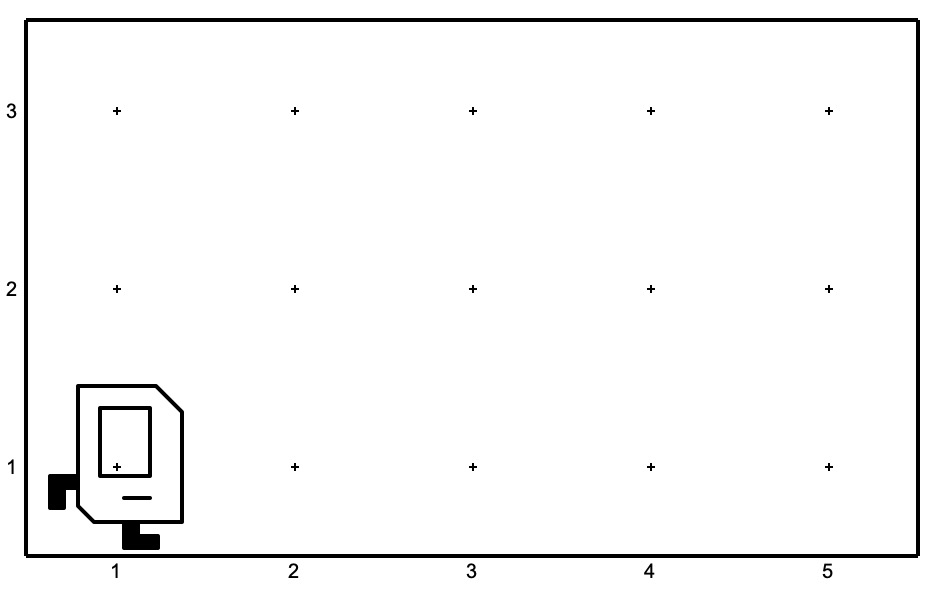
\includegraphics[scale=0.19]{images/ch04/mrofb2/1.jpg}
        \caption{}  
        \label{fig:mrofb2_1}   
    \end{subfigure}
    \begin{subfigure}[t]{{\figpctw}\textwidth}
        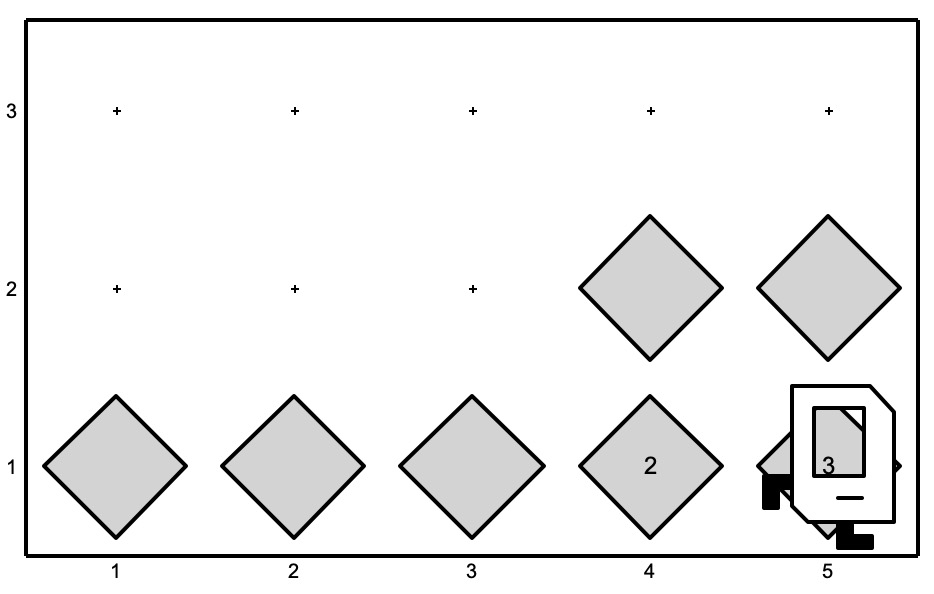
\includegraphics[scale=0.19]{images/ch04/mrofb2/2.jpg}
        \caption{}  
        \label{fig:mrofb2_2}  
    \end{subfigure}
    \caption{}
    \label{fig:mrofb2}
\end{figure}

\section{ရီကားဆစ်ဖ်နည်းဖြင့် ပုစ္ဆာဖြေရှင်းခြင်း}
ရှေ့ စက်ရှင်မှာ လေ့လာခဲ့တာက ရီကားဆစ်ဖ်ဖန်ရှင် ဘယ်လို အလုပ်လုပ်လဲပဲ ရှိပါသေးတယ်။ တစ်နည်း\allowbreak အားဖြင့် မက္ကနစ်ဇမ် \fEn{(mechanism)} ကို လေ့လာတာပါ။ အခုတစ်ခါ ရီကားဆစ်ဖ်ဖန်ရှင်တွေနဲ့ ပုစ္ဆာတွေ ဘယ်လိုဖြေရှင်းမလဲ ဆက်လက်လေ့လာပါမယ်။  ‘ရီကားဆစ်ဖ် စဉ်းစားခြင်း’ \fEn{(thinking recursively}\fEn{)} သို့မဟုတ် ‘ရီကားဆစ်ဖ်နည်းဖြင့် ပုစ္ဆာဖြေရှင်းခြင်း’ \fEn{(solving problems recursively)} ကို လေ့လာမှာပါ။
\subsection*{ရီကားဆစ်ဖ် စဉ်းစားခြင်း ဥပမာ (၁)}
ကွန်နာမှာရှိတဲ့ ဘိပါတွေအားလုံး ကောက်မယ်ဆိုပါစို့။ ဘိပါတစ်ခုနဲ့ အထက်ရှိနိုင်တယ်။ ဘိပါမရှိတာလည်း ဖြစ်နိုင်တယ် ယူဆပါ။ ဒီအတွက် ရီကားဆစ်ဖ်ဖန်ရှင် သတ်မှတ်ပါမယ်။ 
%
\setlength{\fboxsep}{0pt}
\begin{minted}[frame=\mintframe, framerule=\mintrule,framesep= \mintsep, xleftmargin=\xlftmargin
    , bgcolor=mintbgcolor,rulecolor=mintrulecolor
    , python3=true,escapeinside=ßß]{python}
def pick_all_beepers():
    ... # ß\fEn{to do soon}ß
\end{minted}
%

ဖြေရှင်းမဲ့ကိစ္စတစ်ခုကို ၎င်းကိုယ်တိုင်နဲ့ ပုံပန်းသဏ္ဌာန်တူပြီး အရွယ်အစားအားဖြင့် တစ်ဆင့်ထက်တစ်ဆင့် သေးငယ်တဲ့ ကိစ္စတွေအဖြစ် ခွဲခြမ်းကြည့်ပါတယ်။ ဥပမာ ဘိပါငါးခုရှိတဲ့ ကိစ္စကို ဘိပါလေးခု၊ သုံးခု၊ နှစ်ခု နဲ့ တစ်ခု ရှိတဲ့ ကိစ္စတွေအဖြစ် ခွဲပြီး မြင်ကြည့်ရမှာပါ။ ဒီကိစ္စမှာ ဘိပါအရေအတွက်ဟာ အရွယ်အစားပဲ။ လေးခုရှိတဲ့ ကိစ္စဟာ ငါးခုရှိတဲ့ကိစ္စထက် အရွယ်အားဖြင့် တစ်ဆင့်ငယ်တာပေါ့။ ဘိပါမရှိတာလည်း ဖြစ်နိုင်တော့ သုညဘိပါဟာ အငယ်ဆုံးဖြစ်တယ်လို့ ယူဆနိုင်တယ်။

\fCode{pick\_all\_beepers} ဖန်ရှင်ဟာ လက်ရှိဖြေရှင်းမဲ့ အရွယ်အစားထက် တစ်ဆင့်ငယ်တဲ့ ကိစ္စကို ဖြေရှင်းနိုင်ပြီးသားလို့ မှတ်ယူရပါမယ်။ လက်ရှိဖြေရှင်းမဲ့ ကိစ္စက ဘိပါငါးခု ကောက်ရမယ်ဆိုရင် ဘိပါလေးခု ကောက်နိုင်ပြီးသားလို့ ယူဆရမှာပါ။ $n$ ဘိပါရှိတယ် ဆိုရင် $n - 1$ ဘိပါကို ကောက်နိုင်ပြီးသား ယူဆရမယ်။ \fEn{Top-down} နည်းမှာလည်း ဒီလိုပဲ မရှိသေးဘဲ၊ မလုပ်နိုင်သေးဘဲ ရှိတယ်၊ လုပ်နိုင်တယ် မှတ်ယူပြီး စဉ်းစားဖြေရှင်းတာကို ပြန်အမှတ်ရမှာပါ။ ရီကားဆစ်ဖ် စဉ်းစားတဲ့အခါမှာ လက်ရှိသတ်မှတ်နေတဲ့ ဖန်ရှင်ကိုယ်တိုင်ကို ရှိပြီးဖြစ်တယ်လို့ သဘောထားရတာ။

ပြီးတဲ့အခါ လက်ရှိကိစ္စကနေ သူ့ထက်တစ်ဆင့်ငယ်တဲ့ ကိစ္စဖြစ်သွားအောင် ဘာလုပ်ရမလဲ စဉ်းစားရတယ်။ ဘိပါငါးခုကနေ လေးခုဖြစ်အောင် ဘိပါတစ်ခု ကောက်ရမှာပေါ့။ ယျေဘုယျပြောရင် $n$ ဘိပါရှိရင် ဆိုရင် $n - 1$ ဘိပါဖြစ်သွားအောင် ဘာလုပ်ရမလဲ စဉ်းစားတာ။

လက်ရှိဖန်ရှင်ဟာ $n - 1$ ဘိပါကို ကောက်နိုင်ပြီးသားလို့ ယူဆထားတယ်။  $n$ ဘိပါရှိရင် ဘိပါတစ်ခု ကောက်လိုက်ရင် $n - 1$ ဘိပါဖြစ်သွားမယ်။  ကျန်နေတဲ့  $n - 1$ ဘိပါကောက်ဖို့ လက်ရှိဖန်ရှင်ကိုပဲ ပြန်ခေါ်လိုက်မှာပေါ့။
%
\setlength{\fboxsep}{0pt}
\begin{minted}[frame=\mintframe, framerule=\mintrule,framesep= \mintsep, xleftmargin=\xlftmargin
    , bgcolor=mintbgcolor,rulecolor=mintrulecolor
    , python3=true,escapeinside=ßß]{python}
# ß\fEn{only partially done}ß
def pick_all_beepers():
    ...
    # ß\fEn{to pick $(n)$ beepers}ß
    pick_beeper()
    pick_all_beepers() # ß\fEn{assuming it can pick $(n - 1)$ beepers}ß
    ...
\end{minted}
%
ရီကားဆစ်ဖ် စဉ်းစားတတ်ဖို့ ဒီအဆင့်က အခရာအကျဆုံးပဲ။ တစ်ဆင့်ငယ်တဲ့ ကိစ္စ $n - 1$ ကို ဖြေရှင်းနိုင်ပြီးသားလို့ မှတ်ယူပြီး လက်ရှိကစ္စ $n$ ကို ဘယ်လို ဖြေရှင်းမလဲ စဉ်းစားသွားတာ။

ဖန်ရှင်သတ်မှတ်ချက်က မပြီးသေးပါဘူး။ အသေးငယ်ဆုံး ကိစ္စကို ချွင်းချက်အနေနဲ့ စဉ်းစားရမယ်။  အသေးငယ်ဆုံးကိစ္စက ဘိပါမရှိတာ (သုည) ဖြစ်တယ်။ ဘိပါမရှိရင် ဘာမှလုပ်စရာမလိုဘူး။ $n$ နဲ့ $n - 1$ ဘိပါအတွက် အထက်ပါအတိုင်း စဉ်းစားတဲ့အခါ $n \neq 0$ လို့ ယူဆရမှာပါ။ ဒါကြောင့် ဘိပါရှိမှပဲ လုပ်အောင် အခုလိုဖြစ်ရပါမယ်

%
\setlength{\fboxsep}{0pt}
\begin{minted}[frame=\mintframe, framerule=\mintrule,framesep= \mintsep, xleftmargin=\xlftmargin
    , bgcolor=mintbgcolor,rulecolor=mintrulecolor
    , python3=true,escapeinside=ßß]{python}
# ß\fEn{finished}ß
def pick_all_beepers():
    if beepers_present():
        pick_beeper()
        pick_all_beepers()
\end{minted}
%


\subsection*{ရီကားဆစ်ဖန်ရှင် မှန်မမှန် စစ်ဆေးခြင်း}
ရီကားဆစ်ဖန်ရှင် တက်စ် \fEn{(test)} လုပ်ရင် အသေးဆုံးကိစ္စကနေ စရတယ်။ ပြီးခဲတဲ့ ဖန်ရှင်အတွက် အသေးဆုံးက သုညပါ။ ဘိပါမရှိရင် ဖန်ရှင်က မှန်ရဲ့လား အရင်ဆုံး စစ်ကြည့်ပါမယ်။

%
\setlength{\fboxsep}{0pt}
\begin{minted}[frame=\mintframe, framerule=\mintrule,framesep= \mintsep, xleftmargin=\xlftmargin
    , bgcolor=mintbgcolor,rulecolor=mintrulecolor
    , python3=true,escapeinside=ßß]{python}
# ß\fEn{assume no beeper}ß
pick_all_beepers()
\end{minted}
%
\fCode{if} ဘလောက် မလုပ်ဆောင်ဘဲ \fEn{return} ဖြစ်သွားမှာပါ (ရီကားဆစ်ဖ်ကောလ် မဖြစ်လိုက်ဘူး)။ သုညဘိပါအတွက် ဖြစ်သင့်တဲ့အတိုင်း ဖြစ်ပါတယ်။ ဘိပါတစ်ခုပဲ ရှိရင်ရော ဘယ်လိုဖြစ်မလဲ။ ဘိပါကောက်တယ် သုညဘိပါဖြစ်သွားပြီး ရီကားဆစ်ဖ်ကောလ် ဖြစ်မယ်။ တစ်ကြိမ်ပဲ ဖြစ်မယ်။ \fCode{if} ဘလောက် အလုပ်မလုပ်ဘဲ \fEn{return} ပြန်မယ်။
%
\setlength{\fboxsep}{0pt}
\begin{minted}[frame=\mintframe, framerule=\mintrule,framesep= \mintsep, xleftmargin=\xlftmargin
    , bgcolor=mintbgcolor,rulecolor=mintrulecolor
    , python3=true,escapeinside=ßß]{python}
# ß\fEn{initial call}ß
pick_all_beepers()ß\tikzmarknode{h1}ß
    # ß\fEn{1\textsuperscript{\fEn{st}} recur}ß
    pick_all_beepers()ß\tikzmarknode{h2}ß
\end{minted}
\begin{tikzpicture}[
  remember picture,
  overlay,
  annotation/.style={
    inner sep=0pt,
    outer sep=0pt,
    outer xsep=1mm,
    fill=yellow!80!black,
    text width=5cm
  },
  >={Stealth[inset=0pt, angle=30:7pt]}
]
\draw[->, thin] (pic cs:h1)  ++(0,.3ex) .. controls ([xshift=1.1cm,yshift=-.11cm]pic cs:h1) and ([xshift=.5cm,yshift=.5cm]pic cs:h2) ..  ([yshift=1.2ex] pic cs:h2);
\draw[->, thin, red] (pic cs:h2)  ++(0,1ex) .. controls ([xshift=1.7cm,yshift=.4cm]pic cs:h2) and ([xshift=1cm,yshift=.2cm]pic cs:h1) ..  ([yshift=.7ex] pic cs:h1);
%([yshift=0.1em]a.north) to[bend left] ([yshift=0.1em]b.north);}
\end{tikzpicture}%
သုံးခုရှိရင် ရီကားဆစ်ဖ်ကောလ် နှစ်ခါဖြစ်ပြီးမှ \fEn{return} ပြန်မှာပါ။
%
\setlength{\fboxsep}{0pt}
\begin{minted}[frame=\mintframe, framerule=\mintrule,framesep= \mintsep, xleftmargin=\xlftmargin
    , bgcolor=mintbgcolor,rulecolor=mintrulecolor
    , python3=true,escapeinside=ßß]{python}
# ß\fEn{initial call}ß
pick_all_beepers()ß\tikzmarknode{i1}ß
    # ß\fEn{1\textsuperscript{\fEn{st}} recur}ß
    pick_all_beepers()ß\tikzmarknode{i2}ß
        # ß\fEn{2\textsuperscript{\fEn{nd}} recur}ß
        pick_all_beepers()ß\tikzmarknode{i3}ß
\end{minted}
\begin{tikzpicture}[
  remember picture,
  overlay,
  annotation/.style={
    inner sep=0pt,
    outer sep=0pt,
    outer xsep=1mm,
    fill=yellow!80!black,
    text width=5cm
  },
  >={Stealth[inset=0pt, angle=30:7pt]}
]
\draw[->, thin] (pic cs:i1)  ++(0,.3ex) .. controls ([xshift=1.1cm,yshift=-.11cm]pic cs:i1) and ([xshift=.5cm,yshift=.5cm]pic cs:i2) ..  ([yshift=1.2ex] pic cs:i2);
\draw[->, thin] (pic cs:i2)  ++(0,0ex) .. controls ([xshift=1.1cm,yshift=-.11cm]pic cs:i2) and ([xshift=.5cm,yshift=.5cm]pic cs:i3) ..  ([yshift=1.2ex] pic cs:i3);
\draw[->, thin, red] (pic cs:i3)  ++(0,1ex) .. controls ([xshift=1.7cm,yshift=.4cm]pic cs:i3) and ([xshift=1cm,yshift=.2cm]pic cs:i2) ..  ([yshift=.5ex] pic cs:i2);
\draw[->, thin, red] (pic cs:i2)  ++(0,1ex) .. controls ([xshift=1.7cm,yshift=.4cm]pic cs:i2) and ([xshift=1cm,yshift=.2cm]pic cs:i1) ..  ([yshift=.7ex] pic cs:i1);
%([yshift=0.1em]a.north) to[bend left] ([yshift=0.1em]b.north);}
\end{tikzpicture}%
\btwntikzannoandpar


မျှော်လင့်ထားသလို အလုပ်လုပ်နေပါတယ်။ အထက်ပါအတိုင်း စစ်ကြည့်သွားရင် ဘိပါ သုံး၊ လေး၊ ငါး၊ $...$ ခု တွေအတွက်လည်း တောက်လျှောက်မှန်နေမှာပါ။ ဘာကြောင့် ပြောနိုင်ရတာလဲ။ အခုလို စဉ်းစားကြည့်နိုင်ပါတယ်။ ရှေ့မှာ စစ်ကြည့်တာ $n = 0, n = 1$ အတွက် မှန်တာ သေချာပြီ။  $n = 2$ အတွက် စစ်မယ်ဆိုပါစို့
%
\setlength{\fboxsep}{0pt}
\begin{minted}[frame=\mintframe, framerule=\mintrule,framesep= \mintsep, xleftmargin=\xlftmargin
    , bgcolor=mintbgcolor,rulecolor=mintrulecolor
    , python3=true,escapeinside=ßß]{python}
# ß\fEn{start with }$n = 2$ß
if beepers_present():
    pick_beeper() # ß\fEn{after this }$n = 1$ß
    pick_all_beepers() # ß\fEn{works correctly for} $n = 1$ß
\end{minted}
%
$n = 2$ အတွက်မှန်ရင် $n = 3$ အတွက်လည်း ဆက်ပြီး မှန်နေမှာပါ
%
\setlength{\fboxsep}{0pt}
\begin{minted}[frame=\mintframe, framerule=\mintrule,framesep= \mintsep, xleftmargin=\xlftmargin
    , bgcolor=mintbgcolor,rulecolor=mintrulecolor
    , python3=true,escapeinside=ßß]{python}
# ß\fEn{start with }$n = 3$ß
if beepers_present():
    pick_beeper() # ß\fEn{after this }$n = 2$ß
    pick_all_beepers() # ß\fEn{already works for} $n = 2$ß
\end{minted}
%
$n = 3$ အတွက်မှန်ရင် $n = 4$ အတွက်လည်း မှန်ပြီပေါ့
%
\setlength{\fboxsep}{0pt}
\begin{minted}[frame=\mintframe, framerule=\mintrule,framesep= \mintsep, xleftmargin=\xlftmargin
    , bgcolor=mintbgcolor,rulecolor=mintrulecolor
    , python3=true,escapeinside=ßß]{python}
# ß\fEn{start with }$n = 4$ß
if beepers_present():
    pick_beeper() # ß\fEn{after this }$n = 3$ß
    pick_all_beepers() # ß\fEn{already works for} $n = 3$ß
\end{minted}
%
ဒီတိုင်းဆက်သွားရင် သုညအပါအဝင် မည်သည့် အပေါင်းကိန်းပြည့် $n$ အတွက်မဆို \fEn{(non-negative integer)}  မှန်တယ်ဆိုတာ မြင်နိုင်ပါတယ်။












\subsection*{ရီကားဆစ်ဖ် စဉ်းစားခြင်း ဥပမာ (၂)}
ဒုတိယ ဥပမာအနေနဲ့ အခန်း (၃) က အမှိုက်ရှင်းတဲ့ ဥပမာကို ရီကားဆစ်ဖ်နည်းနဲ့ ဖြေရှင်းကြည့်ရအောင်။ လမ်းတစ်လမ်းရှင်းဖို့ ဘယ်လိုစဉ်းစားမလဲ။
\begin{mytcbox}
ဖြေရှင်းမဲ့ကိစ္စကို ၎င်းကိုယ်တိုင်နဲ့ သဏ္ဌာန်တူပြီး အရွယ်အစားအားဖြင့် တစ်ဆင့်ထက်တစ်ဆင့် သေးငယ်တဲ့ ကိစ္စတွေအဖြစ် ခွဲခြမ်းကြည့်ရမှာပါ။
\end{mytcbox}%

လမ်းတစ်ခုရဲ့ အရှည်ကို အရွယ်အစားလို့ ယူဆနိုင်တယ်။ တစ်နည်းအားဖြင့် လမ်းတစ်လျှောက် ကွန်နာအရေအတွက်ဟာ အခုဖြေရှင်းမဲ့ ကိစ္စရဲ့ အရွယ်အစားပဲ။ ကွန်နာတစ်ခုတော့ အနည်းဆုံး ရှိရမယ်။ ဒါကြောင့် အသေးဆုံးက $n = 1$ ဖြစ်တယ်။

\begin{mytcbox}
\fCode{clean\_street} ဖန်ရှင်ဟာ လက်ရှိဖြေရှင်းမဲ့ အရွယ်အစားထက် တစ်ဆင့်ငယ်တဲ့ ကိစ္စကို ဖြေရှင်းနိုင်ပြီးသားလို့ မှတ်ယူရပါမယ်။ 
\end{mytcbox}%

အခုကိစ္စအတွက် ကွန်နာငါးခု ရှင်းမယ်ဆိုရင် \fCode{clean\_street} ဖန်ရှင်ဟာ ကွန်နာလေးခုနဲ့ လမ်းကို ရှင်းနိုင်တယ်လို့ ယူဆရမယ်။  $n$ ကွန်နာရှိတဲ့လမ်းအတွက် $n - 1$ ကွန်နာကို ရှင်းနိုင်ပြီးသားလို့ ယူဆရမှာ ဖြစ်ပါတယ်။


\begin{mytcbox}
လက်ရှိအရွယ်အစားကို သူ့ထက်တစ်ဆင့်ငယ်တဲ့ ကိစ္စဖြစ်သွားအောင် ဘာလုပ်ရမလဲ စဉ်းစားရတယ်။ ကွန်နာငါးခု လမ်းကိုရှင်းတဲ့အခါ ကွန်နာ လေးခုပဲ ရှင်းစရာကျန်အောင် ဘာလုပ်မလဲ။ ယျေဘုယျပြောရင် $n$ ကွန်နာဆိုရင် $n - 1$ ကွန်နာ ရှင်းဖို့လိုတော့အောင် ဘာလုပ်မလဲ။ 
\end{mytcbox}%

လမ်းတစ်လမ်းရှင်းတဲ့အခါ လမ်းအစ သို့မဟုတ် လမ်းအဆုံးမှာ အခြားဘက်စွန်းကို  မျက်နှာမူထားတယ်။ ရှေ့တစ်ကွန်နာ ရွှေ့လိုက်ရင်  ရှင်းစရာ ကွန်နာတစ်ခု လျော့သွားမှာပါ။

\begin{mytcbox}
တစ်ဆင့်ငယ်တဲ့ ကိစ္စ $n - 1$ ကို ဖြေရှင်းနိုင်ပြီးသားလို့ မှတ်ယူပြီး လက်ရှိကစ္စ $n$ ကို ဘယ်လို ဖြေရှင်းမလဲ စဉ်းစားရပါမယ်။
\end{mytcbox}%

ကွန်နာငါးခုရှင်းမယ်ဆိုရင် လေးခုကို ရှင်းနိုင်ပြီးသား မှတ်ယူထားရမယ်။ ဘိပါရှိရင်ကောက်၊ ရှေ့တစ်ကွန်နာ ရွှေ့ထားလိုက်ရင် ရှင်းစရာ လေးခုပဲကျန်မယ်။ ဒီလေးခုကို လက်ရှိသတ်မှတ်နေတဲ့ ဖန်ရှင်နဲ့ ရှင်းလိုက်ရုံပဲပေါ့။
%
\setlength{\fboxsep}{0pt}
\begin{minted}[frame=\mintframe, framerule=\mintrule,framesep= \mintsep, xleftmargin=\xlftmargin
    , bgcolor=mintbgcolor,rulecolor=mintrulecolor
    , python3=true,escapeinside=ßß]{python}
def clean_street():
    ...
    if beepers_present():
        pick_beeper()
    move()
    clean_street() # ‌ß\fEn{assuming already works for $n - 1$}ß
    ...
\end{minted}
%
\begin{mytcbox}
    အသေးငယ်ဆုံး ကိစ္စကို ချွင်းချက်အနေနဲ့ စဉ်းစားရမယ်။   ကွန်နာတစ်ခုဟာ အသေးငယ်ဆုံးကိစ္စ ဖြစ်တယ်။ ဒီကိစ္စကို ဘယ်လိုဖြေရှင်းမလဲ။
\end{mytcbox}

ကွန်နာတစ်ခုပဲ ရှိတယ်ဆိုရင် ဘိပါရှိရင် ကောက်လိုက်ရုံပါပဲ။ $n$ နဲ့ $n - 1$ ကွန်နာ အတွက် အထက်ပါအတိုင်း စဉ်းစားတဲ့အခါ $n > 1$ လို့ ယူဆရမှာပါ။ ရှေ့မှာရှင်းနေရင် $n > 1$ မို့လို့၊ မရှင်းတော့ဘူးဆိုရင် $n = 1$ ဖြစ်နေပြီ။
%
\setlength{\fboxsep}{0pt}
\begin{minted}[frame=\mintframe, framerule=\mintrule,framesep= \mintsep, xleftmargin=\xlftmargin
    , bgcolor=mintbgcolor,rulecolor=mintrulecolor
    , python3=true,escapeinside=ßß]{python}
def clean_street():
    if front_is_clear():       # ß\fMM{ရှေ့မှာ ကွန်နာတွေ ရှိနေသေးရင်}ß
        if beepers_present():
            pick_beeper()
        move()
        clean_street()
    else:                      # ß\fMM{နောက်ဆုံးကွန်နာဆိုရင်}ß
        if beepers_present():
            pick_beeper() 
\end{minted}
အသေးဆုံးကနေစပြီး ဖန်ရှင် အလုပ်လုပ်တာ မှန်/မမှန် စိစစ်ပါ။ ကွန်နာတစ်ခုပဲ ရှိတဲ့လမ်းဆိုရင် စစချင်းပဲ ရှေ့မှာ ပိတ်နေမှာပါ။ \fCode{else} အပိုင်း အလုပ်လုပ်မယ်။ ဘိပါရှိရင် ကောက်တယ်။ ကွန်နာနှစ်ခု ရှိတယ်ဆိုရင် စစချင်း ရှေ့မှာ နံရံမရှိဘူး။ \fCode{if} အပိုင်း အလုပ်လုပ်မယ်။ ဘိပါရှိရင် ကောက်တယ်၊ ရှေ့တိုးတယ် (နံရံပိတ်သွားပြီ)။  ရီကားဆစ်ဖ်ကောလ် ဖြစ်တယ်။ \fCode{else} အပိုင်းလုပ်ပြီးတာနဲ့ \fEn{return} စဖြစ်တယ်။

ဒီအတိုင်းဆက်စစ်သွားရင် တစ်ခုထက်ပိုတဲ့ ကွန်နာတွေအတွက်လည်း မှန်အောင် အလုပ်လုပ်နေမယ်ဆိုတာ သက်သေပြနိုင်ပါတယ်။ စာရေးသူ အတွေ့အကြုံအရ အသေးဆုံးနဲ့ သူ့ထက်ကြီးတာ နှစ်ခုသုံးခုလောက်ထိ မှန်တယ်ဆိုရင် နောက်ဟာတွေအတွက် မှားစရာ အကြောင်းမရှိတော့ဘူး။

ရီကားဆစ်ဖ်နည်းနဲ့ လမ်းတစ်လမ်း ရှင်းလို့ရပါပြီ။ ကားရဲလ်ကမ္ဘာတစ်ခုလုံး ရှင်းဖို့ ရီကားဆစ်ဖ် ဆက်ပြီး စဉ်းစားပါမယ်။ 
%
\begin{itemize}
    \item လမ်းအရေအတွက်ဟာ အရွယ်အစားလို့ ယူဆနိုင်တယ်။ အသေးဆုံးက လမ်းတစ်လမ်းပါ။
    \item ငါးလမ်းရှိရင် ကျန်တဲ့လေးလမ်းကို ရှင်းနိုင်ပြီးသား မှတ်ယူရမယ်။
    \item (၁) လမ်းရှင်းပြီး အဆုံးမှာ အပေါ်လမ်း ကူးလိုက်ရင် လေးလမ်းပဲကျန်မယ် (လမ်းအရေအတွက် $n$ ရှိရာကနေ   $n - 1$ ဖြစ်အောင် ဘာလုပ်မလဲ စဉ်းစားတာ)။
    \item တစ်ဆင့်ငယ်တဲ့ ကိစ္စ $n - 1$ ကို ဖြေရှင်းနိုင်ပြီးသားလို့ မှတ်ယူပြီး လက်ရှိကစ္စ $n$ ကို ဘယ်လို ဖြေရှင်းမလဲ စဉ်းစားရပါမယ်။
%
\setlength{\fboxsep}{0pt}
\begin{minted}[frame=\mintframe, framerule=\mintrule,framesep= \mintsep, xleftmargin=\xlftmargin
    , bgcolor=mintbgcolor,rulecolor=mintrulecolor
    , python3=true,escapeinside=ßß]{python}
def clean_world():
    ...
    clean_street()
    turn_north()
    change_street()
    clean_world()
    ...
\end{minted}
    တစ်လမ်းရှင်းပြီး နောက်တစ်လမ်းကို ကူးလိုက်ရင် ဆက်ရှင်းဖို့ လမ်း အရေအတွက် $n - 1$ ကျန်မယ် (ငါးလမ်းရှိတာကို တစ်လမ်းရှင်းပြီး အပေါ်လမ်းကူးလိုက်ရင် ရှင်းစရာ လမ်း လေးခုပဲ ကျန်မယ်) ။ ကျန်တဲ့ $n - 1$  လမ်းကို ရှင်းဖို့ လက်ရှိ \fCode{clean\_world} ဖန်ရှင်ကိုပဲ ပြန်ခေါ်တယ်။
%
    \item အသေးငယ်ဆုံး ကိစ္စကို ချွင်းချက်အနေနဲ့ စဉ်းစားရမယ်။   လမ်းတစ်လမ်းပဲရှိတာက အသေးငယ်ဆုံး။ လမ်းတစ်လမ်းရှင်းပြီး မြောက်ဘက်လှည့်အပြီး ပိတ်နေပြီဆိုရင်တော့ နောက်ထပ် ဆက်ပြီးရှင်းစရာ လမ်းမရှိတော့ဘူး။ အပေါ်အဆင့်က လမ်းကူးတာနဲ့ ကျန်တဲ့လမ်းတွေကို ရှင်းတဲ့ကိစ္စကို မြောက်ဘက်လှည့်ပြီးတဲ့အခါ ရှေ့မှာရှင်းနေမှ လုပ်ရမှာပါ။ ဒီတော့ အခုလို 
    %
\setlength{\fboxsep}{0pt}
\begin{minted}[frame=\mintframe, framerule=\mintrule,framesep= \mintsep, xleftmargin=\xlftmargin
    , bgcolor=mintbgcolor,rulecolor=mintrulecolor
    , python3=true,escapeinside=ßß]{python}
def clean_world():
    clean_street()
    turn_north()
    if front_is_clear():
        change_street()
        clean_world()
\end{minted}
    ဖြစ်ရမယ်။ 
%
\end{itemize}
%
တစ်လမ်း၊ နှစ်လမ်း၊ သုံးလမ်း အသေးဆုံး ကိစ္စတွေ မှန်/မမှန် စိစစ်ကြည့်ပါ။ ပရိုဂရမ် အစအဆုံး ဖော်ပြပေးထားပါတယ်။ လေ့လာကြည့်ပါ။
%
\setlength{\fboxsep}{0pt}
\begin{minted}[frame=\mintframe, framerule=\mintrule,framesep= \mintsep, xleftmargin=\xlftmargin
    , bgcolor=mintbgcolor,rulecolor=mintrulecolor
    , python3=true,escapeinside=ßß]{python}
# File: clean_world_recur1.py
from stanfordkarel import *

def main():
    clean_world()

def clean_world():
    clean_street()
    turn_north()
    if front_is_clear():
        change_street()
        clean_world()

def clean_street():
    if front_is_clear():       # ß\fMM{ရှေ့မှာ ကွန်နာတွေ ရှိနေသေးရင်}ß
        if beepers_present():
            pick_beeper()
        move()
        clean_street()
    else:                      # ß\fMM{နောက်ဆုံးကွန်နာဆိုရင်}ß
        if beepers_present():
            pick_beeper()

def change_street():
    move()
    if right_is_blocked():
        turn_left()
    else:
        turn_right()

def turn_right():
    turn_left()
    turn_left()
    turn_left()

def turn_north():
    while not_facing_north():
        turn_left()

if __name__ == "__main__":
    run_karel_program("clean_world")
\end{minted}
%

%
\setlength{\fboxsep}{0pt}
\begin{minted}[frame=\mintframe, framerule=\mintrule,framesep= \mintsep, xleftmargin=\xlftmargin
    , bgcolor=mintbgcolor,rulecolor=mintrulecolor
    , python3=true,escapeinside=ßß]{python}
# File: checkerboard_recur.py
from stanfordkarel import *

def main():
    mk_checkerboard()

def mk_checkerboard():
    mk_checker_row()
    turn_north()
    if front_is_clear():
        if beepers_present():
            switch_row()
            mk_checker_row2()
        else:
            switch_row()
            mk_checker_row()
        turn_north()
        if front_is_clear():
            switch_row()
            mk_checkerboard()

def mk_checker_row():
    put_beeper()
    if front_is_clear():
        move()
        if front_is_clear():
            move()
            mk_checker_row()

def mk_checker_row2():
    if front_is_clear():
        move()
        put_beeper()
        if front_is_clear():
            move()
            mk_checker_row2()

def switch_row():
    move()
    if right_is_blocked():
        turn_left()
    else:
        turn_right()

def turn_right():
    turn_left()
    turn_left()
    turn_left()

def turn_north():
    while not_facing_north():
        turn_left()

if __name__ == "__main__":
    run_karel_program("4x5")
\end{minted}
%